\section{PRM  Class Reference}
\label{classPRM}\index{PRM@{PRM}}
A probabilistic roadmap planner, proposed by Kavraki, Svestka, Latombe, Overmars, 1994. 


{\tt \#include $<$prm.h$>$}

Inheritance diagram for PRM::\begin{figure}[H]
\begin{center}
\leavevmode
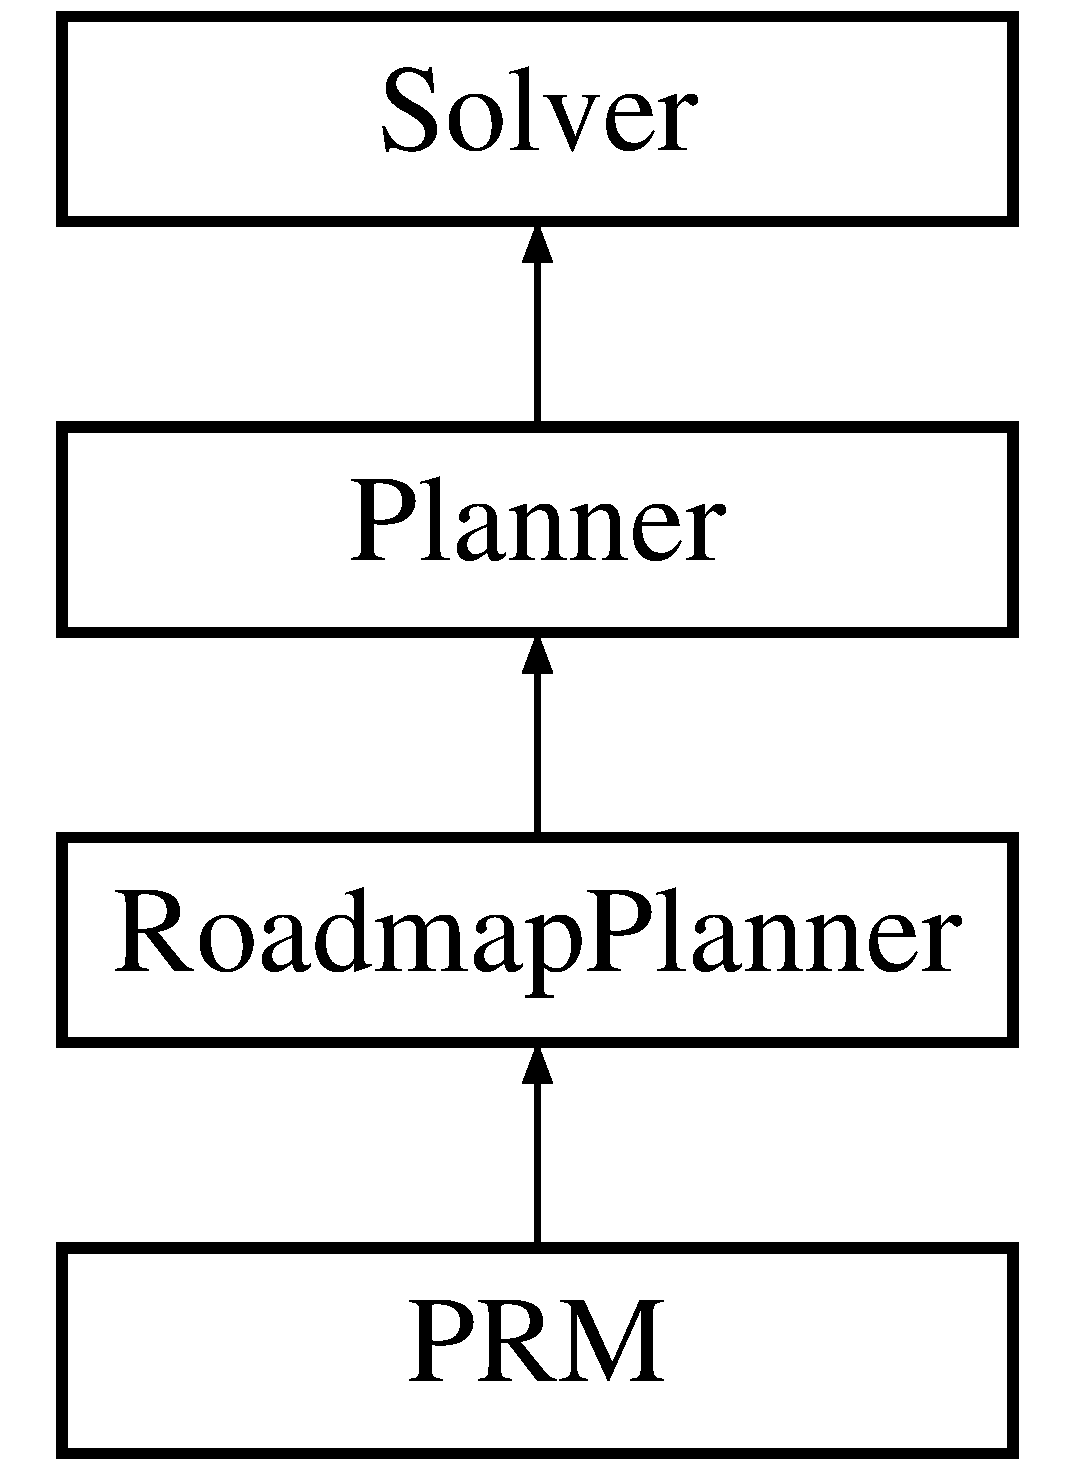
\includegraphics[height=4cm]{classPRM}
\end{center}
\end{figure}
\subsection*{Public Methods}
\begin{CompactItemize}
\item 
{\bf PRM} ({\bf Problem} $\ast$problem)
\begin{CompactList}\small\item\em A constructor that initializes data members.\item\end{CompactList}\item 
virtual {\bf $\sim$PRM} ()
\begin{CompactList}\small\item\em Empty destructor.\item\end{CompactList}\item 
virtual void {\bf Construct} ()
\begin{CompactList}\small\item\em Build a PRM.\item\end{CompactList}\item 
virtual bool {\bf Plan} ()
\begin{CompactList}\small\item\em Try to solve a planning query using an existing PRM.\item\end{CompactList}\end{CompactItemize}
\subsection*{Public Attributes}
\begin{CompactItemize}
\item 
double {\bf Radius}
\begin{CompactList}\small\item\em Used for deciding on which neighbors to choose.\item\end{CompactList}\item 
int {\bf Satisfied\-Count}
\begin{CompactList}\small\item\em Number of times the collision checker has been called.\item\end{CompactList}\item 
bool {\bf Quasi\-Random}
\begin{CompactList}\small\item\em If true, then quasirandom sampling is used (make a file named Quasi\-Random).\item\end{CompactList}\item 
bool {\bf Quasi\-Random\-Hammersley}
\begin{CompactList}\small\item\em Choose Hammersley, over Halton sequence.\item\end{CompactList}\end{CompactItemize}
\subsection*{Protected Methods}
\begin{CompactItemize}
\item 
virtual {\bf list}$<${\bf MSLVertex}$\ast$$>$ {\bf Neighboring\-Vertices} (const {\bf MSLVector} \&x)
\item 
virtual bool {\bf Connect} (const {\bf MSLVector} \&x1, const {\bf MSLVector} \&x2, {\bf MSLVector} \&u)
\item 
virtual {\bf MSLVector} {\bf Choose\-State} (int i, int maxnum, int dim)
\item 
{\bf MSLVector} {\bf Quasi\-Random\-State\-Hammersley} (int i, int maxnum, int dim)
\item 
{\bf MSLVector} {\bf Quasi\-Random\-State\-Halton} (int i, int dim)
\end{CompactItemize}
\subsection*{Protected Attributes}
\begin{CompactItemize}
\item 
double {\bf Step\-Size}
\begin{CompactList}\small\item\em Computed from Delta\-T using the model.\item\end{CompactList}\item 
int {\bf Max\-Neighbors}
\item 
int {\bf Max\-Edges\-Per\-Vertex}
\end{CompactItemize}


\subsection{Detailed Description}
A probabilistic roadmap planner, proposed by Kavraki, Svestka, Latombe, Overmars, 1994.

The base class for planners based on the Probabilistic Roadmap {\bf Planner} {\rm (p.\,\pageref{classPlanner})} (PRM) framework of Kavraki, Svestka, Latombe, Overmars, 1994. In the base class, only Holonomic planning problems can be solved (i.e., standard path planning, without differential constraints). 



\subsection{Constructor \& Destructor Documentation}
\index{PRM@{PRM}!PRM@{PRM}}
\index{PRM@{PRM}!PRM@{PRM}}
\subsubsection{\setlength{\rightskip}{0pt plus 5cm}PRM::PRM ({\bf Problem} $\ast$ {\em problem})}\label{classPRM_a0}


A constructor that initializes data members.

\index{PRM@{PRM}!~PRM@{$\sim$PRM}}
\index{~PRM@{$\sim$PRM}!PRM@{PRM}}
\subsubsection{\setlength{\rightskip}{0pt plus 5cm}PRM::$\sim$PRM ()\hspace{0.3cm}{\tt  [inline, virtual]}}\label{classPRM_a1}


Empty destructor.



\subsection{Member Function Documentation}
\index{PRM@{PRM}!ChooseState@{ChooseState}}
\index{ChooseState@{ChooseState}!PRM@{PRM}}
\subsubsection{\setlength{\rightskip}{0pt plus 5cm}{\bf MSLVector} PRM::Choose\-State (int {\em i}, int {\em maxnum}, int {\em dim})\hspace{0.3cm}{\tt  [protected, virtual]}}\label{classPRM_b2}


\index{PRM@{PRM}!Connect@{Connect}}
\index{Connect@{Connect}!PRM@{PRM}}
\subsubsection{\setlength{\rightskip}{0pt plus 5cm}bool PRM::Connect (const {\bf MSLVector} \& {\em x1}, const {\bf MSLVector} \& {\em x2}, {\bf MSLVector} \& {\em u})\hspace{0.3cm}{\tt  [protected, virtual]}}\label{classPRM_b1}


\index{PRM@{PRM}!Construct@{Construct}}
\index{Construct@{Construct}!PRM@{PRM}}
\subsubsection{\setlength{\rightskip}{0pt plus 5cm}void PRM::Construct ()\hspace{0.3cm}{\tt  [virtual]}}\label{classPRM_a2}


Build a PRM.



Reimplemented from {\bf Planner} {\rm (p.\,\pageref{classPlanner_a3})}.\index{PRM@{PRM}!NeighboringVertices@{NeighboringVertices}}
\index{NeighboringVertices@{NeighboringVertices}!PRM@{PRM}}
\subsubsection{\setlength{\rightskip}{0pt plus 5cm}{\bf list}$<$ {\bf MSLVertex} $\ast$$>$ PRM::Neighboring\-Vertices$<${\bf MSLVertex}$\ast$$>$ (const {\bf MSLVector} \& {\em x})\hspace{0.3cm}{\tt  [protected, virtual]}}\label{classPRM_b0}


\index{PRM@{PRM}!Plan@{Plan}}
\index{Plan@{Plan}!PRM@{PRM}}
\subsubsection{\setlength{\rightskip}{0pt plus 5cm}bool PRM::Plan ()\hspace{0.3cm}{\tt  [virtual]}}\label{classPRM_a3}


Try to solve a planning query using an existing PRM.



Reimplemented from {\bf Planner} {\rm (p.\,\pageref{classPlanner_a4})}.\index{PRM@{PRM}!QuasiRandomStateHalton@{QuasiRandomStateHalton}}
\index{QuasiRandomStateHalton@{QuasiRandomStateHalton}!PRM@{PRM}}
\subsubsection{\setlength{\rightskip}{0pt plus 5cm}{\bf MSLVector} PRM::Quasi\-Random\-State\-Halton (int {\em i}, int {\em dim})\hspace{0.3cm}{\tt  [protected]}}\label{classPRM_b4}


\index{PRM@{PRM}!QuasiRandomStateHammersley@{QuasiRandomStateHammersley}}
\index{QuasiRandomStateHammersley@{QuasiRandomStateHammersley}!PRM@{PRM}}
\subsubsection{\setlength{\rightskip}{0pt plus 5cm}{\bf MSLVector} PRM::Quasi\-Random\-State\-Hammersley (int {\em i}, int {\em maxnum}, int {\em dim})\hspace{0.3cm}{\tt  [protected]}}\label{classPRM_b3}




\subsection{Member Data Documentation}
\index{PRM@{PRM}!MaxEdgesPerVertex@{MaxEdgesPerVertex}}
\index{MaxEdgesPerVertex@{MaxEdgesPerVertex}!PRM@{PRM}}
\subsubsection{\setlength{\rightskip}{0pt plus 5cm}int PRM::Max\-Edges\-Per\-Vertex\hspace{0.3cm}{\tt  [protected]}}\label{classPRM_n2}


\index{PRM@{PRM}!MaxNeighbors@{MaxNeighbors}}
\index{MaxNeighbors@{MaxNeighbors}!PRM@{PRM}}
\subsubsection{\setlength{\rightskip}{0pt plus 5cm}int PRM::Max\-Neighbors\hspace{0.3cm}{\tt  [protected]}}\label{classPRM_n1}


\index{PRM@{PRM}!QuasiRandom@{QuasiRandom}}
\index{QuasiRandom@{QuasiRandom}!PRM@{PRM}}
\subsubsection{\setlength{\rightskip}{0pt plus 5cm}bool PRM::Quasi\-Random}\label{classPRM_m2}


If true, then quasirandom sampling is used (make a file named Quasi\-Random).

\index{PRM@{PRM}!QuasiRandomHammersley@{QuasiRandomHammersley}}
\index{QuasiRandomHammersley@{QuasiRandomHammersley}!PRM@{PRM}}
\subsubsection{\setlength{\rightskip}{0pt plus 5cm}bool PRM::Quasi\-Random\-Hammersley}\label{classPRM_m3}


Choose Hammersley, over Halton sequence.

\index{PRM@{PRM}!Radius@{Radius}}
\index{Radius@{Radius}!PRM@{PRM}}
\subsubsection{\setlength{\rightskip}{0pt plus 5cm}double PRM::Radius}\label{classPRM_m0}


Used for deciding on which neighbors to choose.

\index{PRM@{PRM}!SatisfiedCount@{SatisfiedCount}}
\index{SatisfiedCount@{SatisfiedCount}!PRM@{PRM}}
\subsubsection{\setlength{\rightskip}{0pt plus 5cm}int PRM::Satisfied\-Count}\label{classPRM_m1}


Number of times the collision checker has been called.

\index{PRM@{PRM}!StepSize@{StepSize}}
\index{StepSize@{StepSize}!PRM@{PRM}}
\subsubsection{\setlength{\rightskip}{0pt plus 5cm}double PRM::Step\-Size\hspace{0.3cm}{\tt  [protected]}}\label{classPRM_n0}


Computed from Delta\-T using the model.



The documentation for this class was generated from the following files:\begin{CompactItemize}
\item 
{\bf prm.h}\item 
{\bf prm.C}\end{CompactItemize}
